\documentclass[11pt]{article}
\usepackage[margin=1in]{geometry}
\usepackage{graphicx}
\usepackage{booktabs}
\usepackage{hyperref}
\usepackage{enumitem}

\title{Geminio Project: Phase 1 \& 2 Summary Report}
\author{Dan Zimmerman \\ Advisor: Dr. Ahmed Imteaj}
\date{\today}

\begin{document}
\maketitle

\section{Phase 1: Paper Review}

The ICCV 2025 paper \textit{``Geminio: Language-Guided Gradient Inversion Attacks in Federated Learning''} by Jiao et al.\ introduces a novel attack that exploits Vision-Language Models (VLMs) to enable \textbf{targeted} gradient inversion in federated learning (FL).

\subsection{Key Concepts}

\begin{itemize}[nosep]
    \item \textbf{Federated Learning \& Gradient Inversion:} In FL, clients keep data private and share only model gradients. Gradient Inversion Attacks (GIAs) attempt to reconstruct private images from these shared gradients. However, existing GIAs fail when the client's batch size is large ($\geq$64 images), because the gradient signal from individual images becomes too diluted.

    \item \textbf{Geminio's Approach:} A malicious FL server uses CLIP (a vision-language model) to compute similarity between each training image's embedding and a natural language query (e.g., ``Any human faces''). The server then trains a malicious global model whose loss surface is reshaped so that images matching the query produce dominant gradients, while non-matching images are suppressed.

    \item \textbf{Loss Surface Reshaping:} The training objective is $\mathcal{L} = \mathbb{E}[\ell_i \cdot (1 - p_i)]$, where $\ell_i$ is the per-sample classification loss and $p_i$ is the CLIP-based similarity probability for sample $i$ relative to the query. This causes the model to amplify gradients from query-relevant samples.

    \item \textbf{Task-Agnostic Targeting:} The same framework supports arbitrary natural language queries---from objects (``jewelry'', ``guns'') to people (``human faces'', ``males with a beard'') to complex scenes (``females riding a horse'')---without retraining the VLM.
\end{itemize}

\section{Phase 2: Code Implementation}

\subsection{Pipeline Overview}

The implementation consists of three stages, all of which were successfully executed on the lab's DGX system (NVIDIA H200 GPUs):

\begin{enumerate}[nosep]
    \item \textbf{VLM Embedding Preprocessing:} Generated CLIP (ViT-L/14) embeddings for 50,000 ImageNet validation images and 1,000 class text descriptions. Outputs: \texttt{imagenet-clip-test.pt} (153 MB) and \texttt{imagenet-clip-meta.pt}.

    \item \textbf{Malicious Model Training:} Trained 5 query-specific malicious ResNet34 classifier heads (5 epochs each, Adam optimizer). Parallelized across 5 GPUs for efficiency ($\sim$5 minutes total).

    \item \textbf{Gradient Inversion Attacks:} Ran HFGradInv attack (24,000 iterations) for each of the 5 queries plus a baseline. Parallelized across 6 GPUs ($\sim$45 minutes total).
\end{enumerate}

\subsection{Issues Encountered and Resolved}

\begin{itemize}[nosep]
    \item \textbf{Dependency conflict:} Latest \texttt{transformers} library was incompatible with PyTorch 2.1.2. Fixed by pinning \texttt{transformers==4.36.2}.
    \item \textbf{Data path mismatch:} ImageNet archives were in a subdirectory; the code expected them at a different path. Fixed with symlinks.
    \item \textbf{Missing config file:} The Hydra configuration system required a \texttt{GeminioImageNet.yaml} that was absent from the repo. Created it based on the existing \texttt{ImageNet.yaml}.
    \item \textbf{Class name format bug:} The embedding script failed because \texttt{dataset.classes} returned tuples instead of strings. Fixed by extracting the first element.
\end{itemize}

\subsection{Results}

\begin{table}[h]
\centering
\begin{tabular}{lcc}
\toprule
\textbf{Method / Query} & \textbf{Rec.\ Loss} & \textbf{Improvement vs.\ Baseline} \\
\midrule
Baseline GIA (no query) & 0.1828 & --- \\
\midrule
Geminio: ``Any jewelry'' & 0.0965 & 47.2\% \\
Geminio: ``Any human faces'' & \textbf{0.0750} & \textbf{59.0\%} \\
Geminio: ``Any males with a beard'' & 0.1097 & 40.0\% \\
Geminio: ``Any guns'' & 0.0984 & 46.2\% \\
Geminio: ``Any females riding a horse'' & 0.1222 & 33.2\% \\
\bottomrule
\end{tabular}
\caption{Reconstruction loss comparison (lower is better). All Geminio queries significantly outperform the baseline.}
\end{table}

The baseline attack produces entirely unrecognizable images across all 128 samples. In contrast, Geminio successfully reconstructs identifiable images for samples matching each query, while non-matching samples appear as suppressed gray patches---exactly as predicted by the paper.

\begin{figure}[h]
\centering
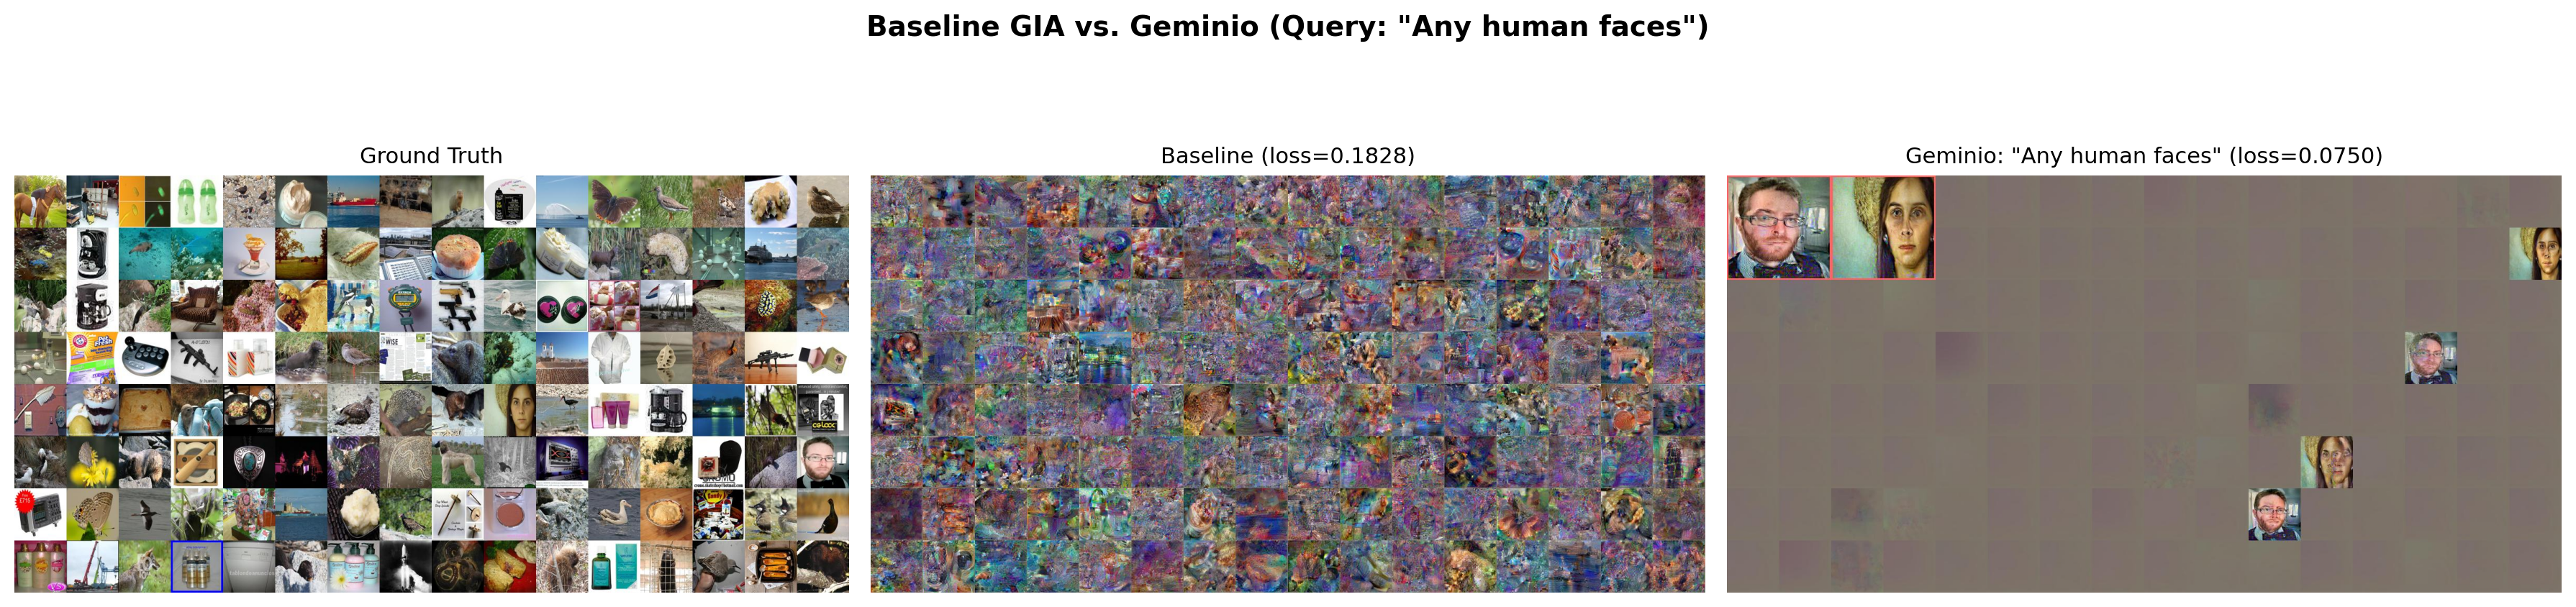
\includegraphics[width=0.95\textwidth]{figures/baseline_vs_geminio.png}
\caption{Ground truth (left), baseline reconstruction (center), and Geminio with query ``Any human faces'' (right). Face images are clearly reconstructed while non-face images are suppressed.}
\end{figure}

\section{Next Steps: Phase 3}

\begin{itemize}[nosep]
    \item \textbf{Healthcare dataset application:} Apply the attack to medical images (MRI, X-ray) provided by Dr. Imteaj and Hossain to test whether patient data can be exposed through gradient inversion despite FL privacy guarantees.
    \item \textbf{VLM adaptation:} Standard CLIP is trained on natural images; a medical VLM (e.g., BiomedCLIP, MedCLIP) may be needed for better image--text alignment on medical data.
    \item \textbf{Defense exploration:} The original paper proposes no defenses. Future work could explore countermeasures such as gradient clipping, differential privacy, or secure aggregation.
\end{itemize}

\end{document}
